\section{Ejercicios Propuestos}

\begin{ejercicio}
\textbf{Ejercicio 1:} Resolución de triángulos rectángulos (cateto y ángulo conocidos)

En cada caso, encuentra todos los elementos del triángulo rectángulo $ABC$ donde $C = 90°$.

\textbf{a)} Si $a = 12$ m (cateto opuesto) y $A = 30°$, encuentra $b$, $c$ y $B$.

\textbf{b)} Si $b = 15$ m (cateto adyacente) y $B = 45°$, encuentra $a$, $c$ y $A$.

\textbf{c)} Si $a = 8$ m (cateto opuesto) y $A = 60°$, encuentra $b$, $c$ y $B$.

\begin{center}
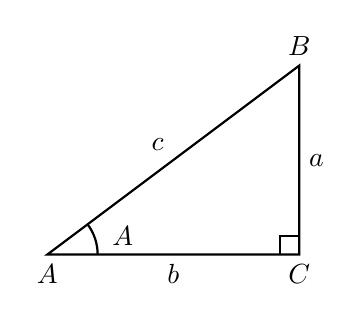
\begin{tikzpicture}[scale=0.8]
    % Triángulo
    \draw[thick] (0,0) -- (4,0) -- (4,3) -- cycle;

    % Ángulo recto
    \draw[thick] (3.7,0) -- (3.7,0.3) -- (4,0.3);

    % Etiquetas
    \node[below] at (0,0) {$A$};
    \node[below] at (4,0) {$C$};
    \node[above] at (4,3) {$B$};
    \node[below] at (2,0) {$b$};
    \node[right] at (4,1.5) {$a$};
    \node[above left] at (2,1.5) {$c$};

    % Ángulos
    \draw[thick] (0.8,0) arc (0:37:0.8);
    \node at (1.2,0.3) {$A$};
\end{tikzpicture}
\end{center}
\end{ejercicio}

\begin{ejercicio}
\textbf{Ejercicio 2:} Resolución de triángulos rectángulos (hipotenusa y ángulo conocidos)

En cada caso, encuentra todos los elementos del triángulo rectángulo $ABC$ donde $C = 90°$.

\textbf{a)} Si $c = 20$ m (hipotenusa) y $A = 30°$, encuentra $a$, $b$ y $B$.

\textbf{b)} Si $c = 10$ m (hipotenusa) y $B = 60°$, encuentra $a$, $b$ y $A$.

\textbf{c)} Si $c = 50$ m (hipotenusa) y $A = 45°$, encuentra $a$, $b$ y $B$.
\end{ejercicio}

\begin{ejercicio}
\textbf{Ejercicio 3:} Ángulo de elevación simple

María observa la parte superior de un edificio desde un punto en el suelo.

\textbf{a)} Si María está a 30 metros del edificio y el ángulo de elevación es de 35°, ¿cuál es la altura del edificio?

\textbf{b)} Si el edificio mide 45 metros de altura y María lo observa con un ángulo de elevación de 52°, ¿a qué distancia del edificio se encuentra María?

\begin{center}
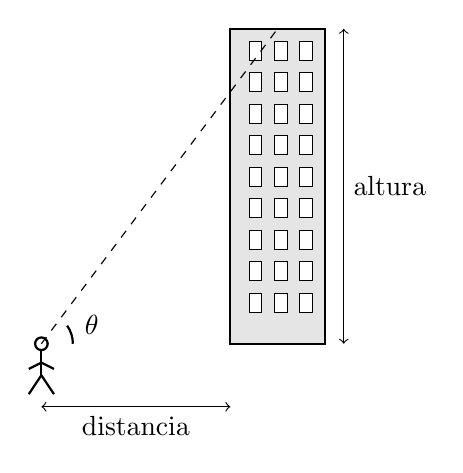
\begin{tikzpicture}[scale=0.08]
    % Edificio
    \draw[thick, fill=gray!20] (0,0) rectangle (15,50);

    % Ventanas
    \foreach \x in {3,7,11}
        \foreach \y in {5,10,15,20,25,30,35,40,45}
            \draw[fill=white] (\x,\y) rectangle (\x+2,\y+3);

    % Persona
    \draw[thick] (-30,0) circle (1);
    \draw[thick] (-30,-1) -- (-30,-5);
    \draw[thick] (-30,-5) -- (-32,-8);
    \draw[thick] (-30,-5) -- (-28,-8);
    \draw[thick] (-30,-3) -- (-32,-4);
    \draw[thick] (-30,-3) -- (-28,-4);

    % Línea de visión
    \draw[dashed] (-30,0) -- (7.5,50);

    % Distancia horizontal
    \draw[<->] (-30,-10) -- (0,-10);
    \node[below] at (-15,-10) {distancia};

    % Ángulo
    \draw[thick] (-25,0) arc (0:35:5);
    \node at (-22,3) {$\theta$};

    % Altura
    \draw[<->] (18,0) -- (18,50);
    \node[right] at (18,25) {altura};
\end{tikzpicture}
\end{center}
\end{ejercicio}

\begin{ejercicio}
\textbf{Ejercicio 4:} Ángulo de depresión simple

Desde lo alto de un acantilado de 80 metros de altura, un observador ve un bote en el mar.

\textbf{a)} Si el ángulo de depresión es de 25°, ¿a qué distancia horizontal del acantilado está el bote?

\textbf{b)} Si el bote está a 120 metros de distancia horizontal del acantilado, ¿cuál es el ángulo de depresión?

\begin{center}
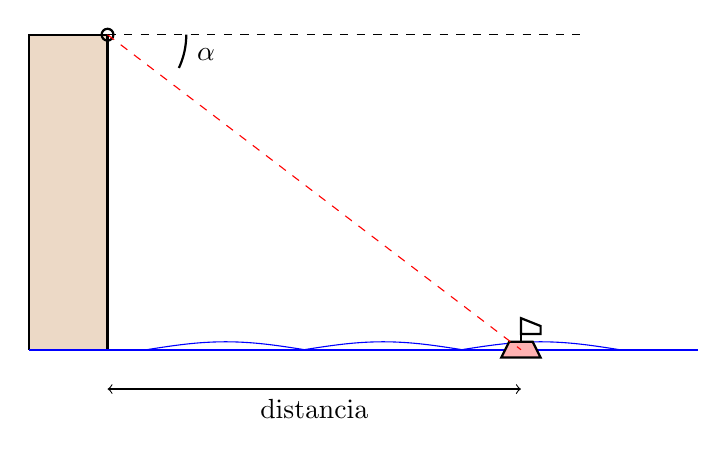
\begin{tikzpicture}[scale=0.05]
    % Acantilado
    \draw[thick, fill=brown!30] (0,0) -- (0,80) -- (-20,80) -- (-20,0);

    % Mar
    \draw[thick, blue] (-20,0) -- (150,0);
    \draw[blue] (10,0) sin (30,2) cos (50,0) sin (70,2) cos (90,0) sin (110,2) cos (130,0);

    % Observador
    \draw[thick] (0,80) circle (1.5);
    \draw[thick] (0,78.5) -- (0,75);

    % Bote
    \draw[thick, fill=red!30] (100,-2) -- (110,-2) -- (108,2) -- (102,2) -- cycle;
    \draw[thick] (105,2) -- (105,8);
    \draw[thick, fill=white] (105,8) -- (110,6) -- (110,4) -- (105,4) -- cycle;

    % Línea de visión
    \draw[dashed, red] (0,80) -- (105,0);

    % Línea horizontal de referencia
    \draw[dashed] (0,80) -- (120,80);

    % Ángulo de depresión
    \draw[thick] (20,80) arc (0:-25:20);
    \node at (25,75) {$\alpha$};

    % Distancia
    \draw[<->] (0,-10) -- (105,-10);
    \node[below] at (52.5,-10) {distancia};
\end{tikzpicture}
\end{center}
\end{ejercicio}

\begin{ejercicio}
\textbf{Ejercicio 5:} Resolver triángulo conociendo dos lados

En cada caso, encuentra todos los ángulos y el lado faltante del triángulo rectángulo $ABC$ donde $C = 90°$.

\textbf{a)} Si $a = 5$ m y $b = 12$ m (catetos), encuentra $c$, $A$ y $B$.

\textbf{b)} Si $a = 15$ m (cateto) y $c = 25$ m (hipotenusa), encuentra $b$, $A$ y $B$.

\textbf{c)} Si $b = 8$ m (cateto) y $c = 10$ m (hipotenusa), encuentra $a$, $A$ y $B$.
\end{ejercicio}

\begin{ejercicio}
\textbf{Ejercicio 6:} Problema aplicado de navegación marítima

Un barco navega desde el puerto $P$ con rumbo N30°E durante 50 km hasta el punto $A$. Luego cambia su rumbo a N60°E y navega 40 km más hasta el punto $B$.

Calcula:
- La distancia en línea recta desde el puerto $P$ hasta el punto final $B$
- El ángulo de dirección desde $P$ hasta $B$ respecto al norte

\begin{center}
\begin{tikzpicture}[scale=0.08]
    % Sistema de coordenadas
    \draw[->] (0,0) -- (0,80) node[above] {N};
    \draw[->] (0,0) -- (80,0) node[right] {E};
    \draw[->] (0,0) -- (0,-20) node[below] {S};
    \draw[->] (0,0) -- (-20,0) node[left] {O};

    % Puerto
    \node[circle, fill=blue, inner sep=2pt] at (0,0) {};
    \node[below left] at (0,0) {$P$};

    % Primera etapa
    \draw[thick, blue, ->] (0,0) -- (25,43.3);
    \node[circle, fill=red, inner sep=2pt] at (25,43.3) {};
    \node[above right] at (25,43.3) {$A$};
    \node[midway, above left] at (12.5,21.65) {50 km};

    % Segunda etapa
    \draw[thick, blue, ->] (25,43.3) -- (59.64,63.3);
    \node[circle, fill=green, inner sep=2pt] at (59.64,63.3) {};
    \node[right] at (59.64,63.3) {$B$};
    \node[midway, above] at (42.32,53.3) {40 km};

    % Línea directa P-B
    \draw[dashed, red, thick] (0,0) -- (59.64,63.3);
    \node[midway, below right] at (29.82,31.65) {$d$};

    % Ángulos
    \draw[thick] (0,15) arc (90:60:15);
    \node at (5,12) {30°};

    \draw[thick] (25,53.3) arc (90:30:10);
    \node at (30,50) {60°};

    % Ángulo desde P a B
    \draw[thick, red] (0,10) arc (90:43:10);
    \node[red] at (5,7) {$\theta$};
\end{tikzpicture}
\end{center}
\end{ejercicio}

\begin{ejercicio}
\textbf{Ejercicio 7:} Problema aplicado de topografía

Un topógrafo necesita medir la altura de una montaña. Desde el punto $A$, a nivel del suelo, observa la cima con un ángulo de elevación de 38°. Avanza 500 metros en línea recta hacia la montaña hasta el punto $B$, y desde allí el ángulo de elevación es de 52°.

Determina:
- La altura de la montaña
- La distancia desde el punto $B$ hasta la base de la montaña

\begin{center}
\begin{tikzpicture}[scale=0.01]
    % Montaña
    \draw[thick, fill=brown!30] plot[smooth] coordinates {(-100,0) (0,0) (100,400) (200,420) (300,450) (400,420) (500,400) (600,0) (700,0)};

    % Cima
    \node[circle, fill=red, inner sep=3pt] at (300,450) {};
    \node[above] at (300,450) {Cima};

    % Punto A
    \node[circle, fill=blue, inner sep=3pt] at (-300,0) {};
    \node[below] at (-300,0) {$A$};

    % Punto B
    \node[circle, fill=blue, inner sep=3pt] at (200,0) {};
    \node[below] at (200,0) {$B$};

    % Base de la montaña
    \node[circle, fill=green, inner sep=3pt] at (300,0) {};
    \node[below] at (300,0) {Base};

    % Líneas de visión
    \draw[dashed, red] (-300,0) -- (300,450);
    \draw[dashed, blue] (200,0) -- (300,450);

    % Distancia A-B
    \draw[<->] (-300,-50) -- (200,-50);
    \node[below] at (-50,-50) {500 m};

    % Altura
    \draw[<->] (350,0) -- (350,450);
    \node[right] at (350,225) {$h$};

    % Ángulos
    \draw[thick] (-250,0) arc (0:38:50);
    \node at (-220,30) {38°};

    \draw[thick] (240,0) arc (0:52:40);
    \node at (265,35) {52°};

    % Distancia B-Base
    \draw[<->] (200,-100) -- (300,-100);
    \node[below] at (250,-100) {$x$};
\end{tikzpicture}
\end{center}
\end{ejercicio}

\begin{ejercicio}
\textbf{Ejercicio 8:} Problema integrador de arquitectura

Un arquitecto está diseñando una escalera de emergencia exterior para un edificio de 4 pisos. Cada piso tiene 3.5 metros de altura. Las normas de seguridad establecen que:
- El ángulo de inclinación debe estar entre 30° y 45°
- Cada tramo de escalera debe tener un descanso
- La proyección horizontal de cada tramo no debe exceder 4 metros

Si el arquitecto decide usar un ángulo de 35° para maximizar la comodidad:

Calcula:
- La longitud de cada tramo de escalera
- La proyección horizontal de cada tramo
- El espacio total horizontal necesario desde el edificio
- El número total de escalones si cada uno tiene 18 cm de altura

\begin{center}
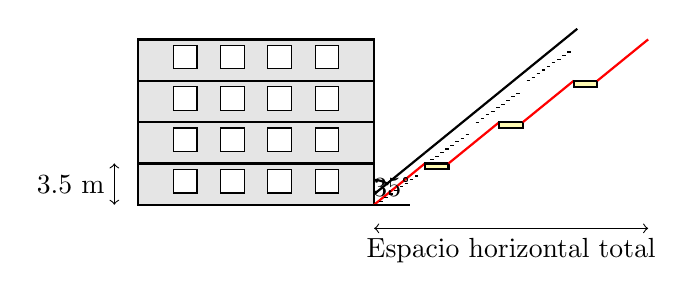
\begin{tikzpicture}[scale=0.15]
    % Edificio
    \draw[thick, fill=gray!20] (0,0) rectangle (20,14);

    % Pisos
    \foreach \y in {3.5,7,10.5}
        \draw[thick] (0,\y) -- (20,\y);

    % Ventanas
    \foreach \x in {3,7,11,15}
        \foreach \y in {1,4.5,8,11.5}
            \draw[fill=white] (\x,\y) rectangle (\x+2,\y+2);

    % Escalera - Tramo 1
    \draw[thick, red] (20,0) -- (24.3,3.5);
    \draw[thick, fill=yellow!30] (24.3,3) rectangle (26.3,3.5);

    % Escalera - Tramo 2
    \draw[thick, red] (26.3,3.5) -- (30.6,7);
    \draw[thick, fill=yellow!30] (30.6,6.5) rectangle (32.6,7);

    % Escalera - Tramo 3
    \draw[thick, red] (32.6,7) -- (36.9,10.5);
    \draw[thick, fill=yellow!30] (36.9,10) rectangle (38.9,10.5);

    % Escalera - Tramo 4
    \draw[thick, red] (38.9,10.5) -- (43.2,14);

    % Proyección horizontal total
    \draw[<->] (20,-2) -- (43.2,-2);
    \node[below] at (31.6,-2) {Espacio horizontal total};

    % Ángulo
    \draw[thick] (20,0) -- (23,0);
    \draw[thick] (20,2.1) arc (90:55:2.1);
    \node at (21.5,1.5) {35°};

    % Altura de piso
    \draw[<->] (-2,0) -- (-2,3.5);
    \node[left] at (-2,1.75) {3.5 m};

    % Pasamanos
    \foreach \i in {1,2,3,4} {
        \draw[thick] (20+4.3*\i-4.3,3.5*\i-3.5+0.9) -- (20+4.3*\i,3.5*\i+0.9);
    }

    % Peldaños (representación simplificada)
    \foreach \i in {0,1,2,3} {
        \foreach \j in {0,0.35,...,3.15} {
            \draw (20+4.3*\i+\j*1.23,3.5*\i+\j*0.87) -- (20+4.3*\i+\j*1.23+0.3,3.5*\i+\j*0.87);
        }
    }
\end{tikzpicture}
\end{center}
\end{ejercicio}

\section{Soluciones de Ejercicios Propuestos}

\begin{solucion}
\textbf{Solución Ejercicio 1:} Resolución de triángulos rectángulos (cateto y ángulo conocidos)

\textbf{a)} Datos: $a = 12$ m, $A = 30°$, $C = 90°$

\textbf{Paso 1: Identificar datos}
\begin{itemize}
    \item Cateto opuesto al ángulo $A$: $a = 12$ m
    \item Ángulo $A = 30°$
    \item Ángulo recto $C = 90°$
\end{itemize}

\textbf{Paso 2: Identificar incógnitas}
\begin{itemize}
    \item Cateto adyacente: $b = ?$
    \item Hipotenusa: $c = ?$
    \item Ángulo $B = ?$
\end{itemize}

\textbf{Paso 3: Encontrar el ángulo $B$}

Como la suma de ángulos en un triángulo es $180°$:
\begin{align*}
A + B + C &= 180° \\
30° + B + 90° &= 180° \\
B &= 180° - 30° - 90° \\
B &= 60°
\end{align*}

\textbf{Paso 4: Encontrar la hipotenusa $c$}

Usando $\sin A = \frac{a}{c}$:
\begin{align*}
\sin 30° &= \frac{12}{c} \\
\frac{1}{2} &= \frac{12}{c} \\
c &= \frac{12}{\frac{1}{2}} \\
c &= 24 \text{ m}
\end{align*}

\textbf{Paso 5: Encontrar el cateto $b$}

Usando $\tan A = \frac{a}{b}$:
\begin{align*}
\tan 30° &= \frac{12}{b} \\
\frac{1}{\sqrt{3}} &= \frac{12}{b} \\
b &= 12\sqrt{3} \\
b &= 12 \times 1.732 \\
b &\approx 20.78 \text{ m}
\end{align*}

\textbf{Paso 6: Verificación}

Teorema de Pitágoras: $a^2 + b^2 = c^2$
\begin{align*}
12^2 + (12\sqrt{3})^2 &= 24^2 \\
144 + 432 &= 576 \\
576 &= 576 \quad \checkmark
\end{align*}

\textbf{Respuesta:} $b = 12\sqrt{3} \approx 20.78$ m, $c = 24$ m, $B = 60°$

\textbf{b)} Datos: $b = 15$ m, $B = 45°$, $C = 90°$

\textbf{Paso 1: Identificar datos}
\begin{itemize}
    \item Cateto adyacente al ángulo $A$: $b = 15$ m
    \item Ángulo $B = 45°$
    \item Ángulo recto $C = 90°$
\end{itemize}

\textbf{Paso 2: Encontrar el ángulo $A$}
\begin{align*}
A + B + C &= 180° \\
A + 45° + 90° &= 180° \\
A &= 45°
\end{align*}

¡Interesante! Es un triángulo isósceles rectángulo.

\textbf{Paso 3: Encontrar el cateto $a$}

Como $A = B = 45°$, entonces $a = b$:
\begin{align*}
a &= 15 \text{ m}
\end{align*}

\textbf{Paso 4: Encontrar la hipotenusa $c$}

Usando $\sin B = \frac{b}{c}$:
\begin{align*}
\sin 45° &= \frac{15}{c} \\
\frac{\sqrt{2}}{2} &= \frac{15}{c} \\
c &= \frac{15 \times 2}{\sqrt{2}} \\
c &= \frac{30}{\sqrt{2}} \times \frac{\sqrt{2}}{\sqrt{2}} \\
c &= \frac{30\sqrt{2}}{2} \\
c &= 15\sqrt{2} \\
c &\approx 21.21 \text{ m}
\end{align*}

\textbf{Verificación:}
\begin{align*}
a^2 + b^2 &= c^2 \\
15^2 + 15^2 &= (15\sqrt{2})^2 \\
225 + 225 &= 450 \\
450 &= 450 \quad \checkmark
\end{align*}

\textbf{Respuesta:} $a = 15$ m, $c = 15\sqrt{2} \approx 21.21$ m, $A = 45°$

\textbf{c)} Datos: $a = 8$ m, $A = 60°$, $C = 90°$

\textbf{Paso 1: Encontrar el ángulo $B$}
\begin{align*}
B &= 180° - 60° - 90° = 30°
\end{align*}

\textbf{Paso 2: Encontrar la hipotenusa $c$}
\begin{align*}
\sin 60° &= \frac{8}{c} \\
\frac{\sqrt{3}}{2} &= \frac{8}{c} \\
c &= \frac{16}{\sqrt{3}} \\
c &= \frac{16\sqrt{3}}{3} \\
c &\approx 9.24 \text{ m}
\end{align*}

\textbf{Paso 3: Encontrar el cateto $b$}
\begin{align*}
\tan 60° &= \frac{8}{b} \\
\sqrt{3} &= \frac{8}{b} \\
b &= \frac{8}{\sqrt{3}} \\
b &= \frac{8\sqrt{3}}{3} \\
b &\approx 4.62 \text{ m}
\end{align*}

\textbf{Verificación:}
\begin{align*}
a^2 + b^2 &= c^2 \\
8^2 + \left(\frac{8\sqrt{3}}{3}\right)^2 &= \left(\frac{16\sqrt{3}}{3}\right)^2 \\
64 + \frac{192}{9} &= \frac{768}{9} \\
\frac{576 + 192}{9} &= \frac{768}{9} \\
\frac{768}{9} &= \frac{768}{9} \quad \checkmark
\end{align*}

\textbf{Respuesta:} $b = \frac{8\sqrt{3}}{3} \approx 4.62$ m, $c = \frac{16\sqrt{3}}{3} \approx 9.24$ m, $B = 30°$
\end{solucion}

\begin{solucion}
\textbf{Solución Ejercicio 2:} Resolución de triángulos rectángulos (hipotenusa y ángulo conocidos)

\textbf{a)} Datos: $c = 20$ m, $A = 30°$, $C = 90°$

\textbf{Paso 1: Encontrar el ángulo $B$}
\begin{align*}
B &= 180° - 30° - 90° = 60°
\end{align*}

\textbf{Paso 2: Encontrar el cateto $a$ (opuesto al ángulo $A$)}
\begin{align*}
\sin 30° &= \frac{a}{20} \\
\frac{1}{2} &= \frac{a}{20} \\
a &= 10 \text{ m}
\end{align*}

\textbf{Paso 3: Encontrar el cateto $b$ (adyacente al ángulo $A$)}
\begin{align*}
\cos 30° &= \frac{b}{20} \\
\frac{\sqrt{3}}{2} &= \frac{b}{20} \\
b &= 10\sqrt{3} \\
b &\approx 17.32 \text{ m}
\end{align*}

\textbf{Verificación:}
\begin{align*}
a^2 + b^2 &= c^2 \\
10^2 + (10\sqrt{3})^2 &= 20^2 \\
100 + 300 &= 400 \\
400 &= 400 \quad \checkmark
\end{align*}

\textbf{Respuesta:} $a = 10$ m, $b = 10\sqrt{3} \approx 17.32$ m, $B = 60°$

\textbf{b)} Datos: $c = 10$ m, $B = 60°$, $C = 90°$

\textbf{Paso 1: Encontrar el ángulo $A$}
\begin{align*}
A &= 180° - 60° - 90° = 30°
\end{align*}

\textbf{Paso 2: Encontrar el cateto $b$ (opuesto al ángulo $B$)}
\begin{align*}
\sin 60° &= \frac{b}{10} \\
\frac{\sqrt{3}}{2} &= \frac{b}{10} \\
b &= 5\sqrt{3} \\
b &\approx 8.66 \text{ m}
\end{align*}

\textbf{Paso 3: Encontrar el cateto $a$ (adyacente al ángulo $B$)}
\begin{align*}
\cos 60° &= \frac{a}{10} \\
\frac{1}{2} &= \frac{a}{10} \\
a &= 5 \text{ m}
\end{align*}

\textbf{Verificación:}
\begin{align*}
a^2 + b^2 &= c^2 \\
5^2 + (5\sqrt{3})^2 &= 10^2 \\
25 + 75 &= 100 \\
100 &= 100 \quad \checkmark
\end{align*}

\textbf{Respuesta:} $a = 5$ m, $b = 5\sqrt{3} \approx 8.66$ m, $A = 30°$

\textbf{c)} Datos: $c = 50$ m, $A = 45°$, $C = 90°$

\textbf{Paso 1: Encontrar el ángulo $B$}
\begin{align*}
B &= 180° - 45° - 90° = 45°
\end{align*}

¡Es un triángulo isósceles rectángulo!

\textbf{Paso 2: Encontrar los catetos $a$ y $b$}

Como $A = B = 45°$, los catetos son iguales:
\begin{align*}
\sin 45° &= \frac{a}{50} \\
\frac{\sqrt{2}}{2} &= \frac{a}{50} \\
a &= \frac{50\sqrt{2}}{2} \\
a &= 25\sqrt{2} \\
a &\approx 35.36 \text{ m}
\end{align*}

Y como es isósceles: $b = a = 25\sqrt{2} \approx 35.36$ m

\textbf{Verificación:}
\begin{align*}
a^2 + b^2 &= c^2 \\
(25\sqrt{2})^2 + (25\sqrt{2})^2 &= 50^2 \\
1250 + 1250 &= 2500 \\
2500 &= 2500 \quad \checkmark
\end{align*}

\textbf{Respuesta:} $a = b = 25\sqrt{2} \approx 35.36$ m, $B = 45°$
\end{solucion}

\begin{solucion}
\textbf{Solución Ejercicio 3:} Ángulo de elevación simple

\textbf{a)} María está a 30 metros del edificio, ángulo de elevación = 35°

\textbf{Paso 1: Identificar el triángulo}

Se forma un triángulo rectángulo donde:
\begin{itemize}
    \item Cateto adyacente = distancia al edificio = 30 m
    \item Cateto opuesto = altura del edificio = $h$ (incógnita)
    \item Ángulo de elevación = 35°
\end{itemize}

\textbf{Paso 2: Elegir la razón trigonométrica}

Como conocemos el cateto adyacente y buscamos el cateto opuesto, usamos la tangente:
\begin{align*}
\tan 35° &= \frac{\text{altura}}{\text{distancia}} \\
\tan 35° &= \frac{h}{30}
\end{align*}

\textbf{Paso 3: Resolver para $h$}
\begin{align*}
h &= 30 \times \tan 35° \\
h &= 30 \times 0.7002 \\
h &= 21.01 \text{ metros}
\end{align*}

\textbf{Respuesta:} El edificio tiene una altura de aproximadamente 21.01 metros.

\textbf{b)} Edificio de 45 metros, ángulo de elevación = 52°

\textbf{Paso 1: Identificar el triángulo}
\begin{itemize}
    \item Cateto opuesto = altura del edificio = 45 m
    \item Cateto adyacente = distancia al edificio = $d$ (incógnita)
    \item Ángulo de elevación = 52°
\end{itemize}

\textbf{Paso 2: Elegir la razón trigonométrica}
\begin{align*}
\tan 52° &= \frac{45}{d}
\end{align*}

\textbf{Paso 3: Resolver para $d$}
\begin{align*}
d &= \frac{45}{\tan 52°} \\
d &= \frac{45}{1.2799} \\
d &= 35.16 \text{ metros}
\end{align*}

\textbf{Respuesta:} María se encuentra a aproximadamente 35.16 metros del edificio.
\end{solucion}

\begin{solucion}
\textbf{Solución Ejercicio 4:} Ángulo de depresión simple

\textbf{a)} Altura del acantilado = 80 m, ángulo de depresión = 25°

\textbf{Paso 1: Comprender el ángulo de depresión}

El ángulo de depresión se mide desde la horizontal hacia abajo. En el triángulo rectángulo formado, este ángulo es igual al ángulo de elevación desde el bote hacia el observador (ángulos alternos internos).

\textbf{Paso 2: Identificar el triángulo}
\begin{itemize}
    \item Cateto opuesto = altura del acantilado = 80 m
    \item Cateto adyacente = distancia horizontal = $d$ (incógnita)
    \item Ángulo (en el triángulo) = 25°
\end{itemize}

\textbf{Paso 3: Aplicar la tangente}
\begin{align*}
\tan 25° &= \frac{80}{d} \\
d &= \frac{80}{\tan 25°} \\
d &= \frac{80}{0.4663} \\
d &= 171.59 \text{ metros}
\end{align*}

\textbf{Respuesta:} El bote está a 171.59 metros de distancia horizontal del acantilado.

\textbf{b)} Altura = 80 m, distancia horizontal = 120 m

\textbf{Paso 1: Plantear la ecuación}
\begin{align*}
\tan \alpha &= \frac{80}{120} \\
\tan \alpha &= \frac{2}{3} \\
\tan \alpha &= 0.6667
\end{align*}

\textbf{Paso 2: Encontrar el ángulo}
\begin{align*}
\alpha &= \arctan(0.6667) \\
\alpha &= 33.69°
\end{align*}

\textbf{Respuesta:} El ángulo de depresión es de aproximadamente 33.69°.
\end{solucion}

\begin{solucion}
\textbf{Solución Ejercicio 5:} Resolver triángulo conociendo dos lados

\textbf{a)} Datos: $a = 5$ m, $b = 12$ m (catetos)

\textbf{Paso 1: Encontrar la hipotenusa $c$}

Usando el Teorema de Pitágoras:
\begin{align*}
c^2 &= a^2 + b^2 \\
c^2 &= 5^2 + 12^2 \\
c^2 &= 25 + 144 \\
c^2 &= 169 \\
c &= 13 \text{ m}
\end{align*}

¡Es una terna pitagórica! (5, 12, 13)

\textbf{Paso 2: Encontrar el ángulo $A$}
\begin{align*}
\tan A &= \frac{a}{b} = \frac{5}{12} \\
A &= \arctan\left(\frac{5}{12}\right) \\
A &= 22.62°
\end{align*}

\textbf{Paso 3: Encontrar el ángulo $B$}
\begin{align*}
B &= 90° - A \\
B &= 90° - 22.62° \\
B &= 67.38°
\end{align*}

\textbf{Verificación:}
\begin{align*}
\sin A &= \frac{5}{13} = 0.3846 \\
\sin 22.62° &= 0.3846 \quad \checkmark
\end{align*}

\textbf{Respuesta:} $c = 13$ m, $A = 22.62°$, $B = 67.38°$

\textbf{b)} Datos: $a = 15$ m, $c = 25$ m

\textbf{Paso 1: Encontrar el cateto $b$}
\begin{align*}
b^2 &= c^2 - a^2 \\
b^2 &= 25^2 - 15^2 \\
b^2 &= 625 - 225 \\
b^2 &= 400 \\
b &= 20 \text{ m}
\end{align*}

¡Otra terna pitagórica! (15, 20, 25) o (3, 4, 5) multiplicada por 5.

\textbf{Paso 2: Encontrar el ángulo $A$}
\begin{align*}
\sin A &= \frac{a}{c} = \frac{15}{25} = \frac{3}{5} = 0.6 \\
A &= \arcsin(0.6) \\
A &= 36.87°
\end{align*}

\textbf{Paso 3: Encontrar el ángulo $B$}
\begin{align*}
B &= 90° - 36.87° = 53.13°
\end{align*}

\textbf{Respuesta:} $b = 20$ m, $A = 36.87°$, $B = 53.13°$

\textbf{c)} Datos: $b = 8$ m, $c = 10$ m

\textbf{Paso 1: Encontrar el cateto $a$}
\begin{align*}
a^2 &= c^2 - b^2 \\
a^2 &= 10^2 - 8^2 \\
a^2 &= 100 - 64 \\
a^2 &= 36 \\
a &= 6 \text{ m}
\end{align*}

¡Terna pitagórica (6, 8, 10) o (3, 4, 5) multiplicada por 2!

\textbf{Paso 2: Encontrar el ángulo $A$}
\begin{align*}
\sin A &= \frac{a}{c} = \frac{6}{10} = 0.6 \\
A &= \arcsin(0.6) \\
A &= 36.87°
\end{align*}

\textbf{Paso 3: Encontrar el ángulo $B$}
\begin{align*}
\cos B &= \frac{b}{c} = \frac{8}{10} = 0.8 \\
B &= \arccos(0.8) \\
B &= 53.13°
\end{align*}

\textbf{Verificación:} $A + B = 36.87° + 53.13° = 90°$ ✓

\textbf{Respuesta:} $a = 6$ m, $A = 36.87°$, $B = 53.13°$
\end{solucion}

\begin{solucion}
\textbf{Solución Ejercicio 6:} Problema aplicado de navegación marítima

\textbf{Paso 1: Establecer sistema de coordenadas}

Colocamos el puerto $P$ en el origen $(0, 0)$, con el norte hacia arriba (eje $y$ positivo) y el este hacia la derecha (eje $x$ positivo).

\textbf{Paso 2: Primera etapa - De $P$ a $A$}

Rumbo N30°E significa 30° desde el norte hacia el este.
\begin{itemize}
    \item Distancia: 50 km
    \item Componente este: $x_A = 50 \sin 30° = 50 \times 0.5 = 25$ km
    \item Componente norte: $y_A = 50 \cos 30° = 50 \times \frac{\sqrt{3}}{2} = 25\sqrt{3} \approx 43.3$ km
\end{itemize}

Posición de $A$: $(25, 43.3)$ km

\textbf{Paso 3: Segunda etapa - De $A$ a $B$}

Rumbo N60°E significa 60° desde el norte hacia el este.
\begin{itemize}
    \item Distancia: 40 km
    \item Componente este desde $A$: $\Delta x = 40 \sin 60° = 40 \times \frac{\sqrt{3}}{2} = 20\sqrt{3} \approx 34.64$ km
    \item Componente norte desde $A$: $\Delta y = 40 \cos 60° = 40 \times 0.5 = 20$ km
\end{itemize}

Posición de $B$:
\begin{align*}
x_B &= x_A + \Delta x = 25 + 34.64 = 59.64 \text{ km} \\
y_B &= y_A + \Delta y = 43.3 + 20 = 63.3 \text{ km}
\end{align*}

\textbf{Paso 4: Distancia directa de $P$ a $B$}
\begin{align*}
d_{PB} &= \sqrt{x_B^2 + y_B^2} \\
d_{PB} &= \sqrt{59.64^2 + 63.3^2} \\
d_{PB} &= \sqrt{3556.73 + 4006.89} \\
d_{PB} &= \sqrt{7563.62} \\
d_{PB} &= 86.97 \text{ km}
\end{align*}

\textbf{Paso 5: Ángulo de dirección desde $P$ hasta $B$}
\begin{align*}
\tan \theta &= \frac{x_B}{y_B} = \frac{59.64}{63.3} = 0.9422 \\
\theta &= \arctan(0.9422) \\
\theta &= 43.29°
\end{align*}

El rumbo desde $P$ hasta $B$ es N43.29°E.

\textbf{Verificación alternativa:}

Usando la ley del coseno en el triángulo $PAB$:
\begin{itemize}
    \item Lado $PA = 50$ km
    \item Lado $AB = 40$ km
    \item Ángulo en $A = 150°$ (ángulo exterior entre los dos rumbos: $180° - 30° = 150°$)
\end{itemize}

\begin{align*}
PB^2 &= PA^2 + AB^2 - 2 \cdot PA \cdot AB \cdot \cos(150°) \\
PB^2 &= 50^2 + 40^2 - 2(50)(40)\cos(150°) \\
PB^2 &= 2500 + 1600 - 4000(-0.866) \\
PB^2 &= 4100 + 3464 \\
PB^2 &= 7564 \\
PB &= 86.97 \text{ km} \quad \checkmark
\end{align*}

\textbf{Respuestas:}
\begin{itemize}
    \item Distancia directa $P$ a $B$: 86.97 km
    \item Rumbo desde $P$ hasta $B$: N43.29°E
\end{itemize}
\end{solucion}

\begin{solucion}
\textbf{Solución Ejercicio 7:} Problema aplicado de topografía

\textbf{Paso 1: Establecer las variables}

Sea:
\begin{itemize}
    \item $h$ = altura de la montaña
    \item $x$ = distancia desde el punto $B$ hasta la base
    \item $x + 500$ = distancia desde el punto $A$ hasta la base
\end{itemize}

\textbf{Paso 2: Plantear las ecuaciones}

Desde el punto $B$ (ángulo de 52°):
\begin{align*}
\tan 52° &= \frac{h}{x} \\
h &= x \tan 52° \\
h &= 1.2799x \quad \text{...(1)}
\end{align*}

Desde el punto $A$ (ángulo de 38°):
\begin{align*}
\tan 38° &= \frac{h}{x + 500} \\
h &= (x + 500) \tan 38° \\
h &= 0.7813(x + 500) \quad \text{...(2)}
\end{align*}

\textbf{Paso 3: Igualar las ecuaciones}

Como ambas expresiones son igual a $h$:
\begin{align*}
1.2799x &= 0.7813(x + 500) \\
1.2799x &= 0.7813x + 390.65 \\
1.2799x - 0.7813x &= 390.65 \\
0.4986x &= 390.65 \\
x &= \frac{390.65}{0.4986} \\
x &= 783.54 \text{ metros}
\end{align*}

\textbf{Paso 4: Calcular la altura}

Sustituyendo en la ecuación (1):
\begin{align*}
h &= 1.2799 \times 783.54 \\
h &= 1002.87 \text{ metros}
\end{align*}

\textbf{Paso 5: Verificación}

Comprobemos con la ecuación (2):
\begin{align*}
h &= 0.7813 \times (783.54 + 500) \\
h &= 0.7813 \times 1283.54 \\
h &= 1002.91 \text{ metros} \quad \checkmark
\end{align*}

(La pequeña diferencia se debe al redondeo)

\textbf{Respuestas:}
\begin{itemize}
    \item Altura de la montaña: 1002.87 metros
    \item Distancia desde el punto $B$ hasta la base: 783.54 metros
\end{itemize}
\end{solucion}

\begin{solucion}
\textbf{Solución Ejercicio 8:} Problema integrador de arquitectura

\textbf{Datos del problema:}
\begin{itemize}
    \item Altura total del edificio: $4 \times 3.5 = 14$ metros
    \item Ángulo de inclinación elegido: $35°$
    \item Altura de cada piso: 3.5 metros
    \item Altura de cada escalón: 18 cm = 0.18 m
    \item Restricción: proyección horizontal máxima por tramo = 4 metros
\end{itemize}

\textbf{Parte 1: Análisis de cada tramo}

Como cada piso tiene 3.5 m de altura y usamos un ángulo de 35°:

\textbf{Para un tramo típico (3.5 m de altura):}

Proyección horizontal de un tramo:
\begin{align*}
\tan 35° &= \frac{3.5}{x} \\
x &= \frac{3.5}{\tan 35°} \\
x &= \frac{3.5}{0.7002} \\
x &= 4.998 \text{ m}
\end{align*}

¡Problema! Esto excede los 4 metros permitidos. Necesitamos ajustar el diseño.

\textbf{Solución: Dividir cada piso en dos tramos con descanso intermedio}

Para medio piso (1.75 m de altura):
\begin{align*}
x_{medio} &= \frac{1.75}{\tan 35°} \\
x_{medio} &= \frac{1.75}{0.7002} \\
x_{medio} &= 2.499 \text{ m} < 4 \text{ m} \quad \checkmark
\end{align*}

\textbf{Parte 2: Longitud de cada medio tramo}

Usando el teorema de Pitágoras o la función coseno:
\begin{align*}
\cos 35° &= \frac{x_{medio}}{L_{medio}} \\
L_{medio} &= \frac{2.499}{\cos 35°} \\
L_{medio} &= \frac{2.499}{0.8192} \\
L_{medio} &= 3.051 \text{ m}
\end{align*}

O alternativamente:
\begin{align*}
L_{medio} &= \sqrt{1.75^2 + 2.499^2} \\
L_{medio} &= \sqrt{3.0625 + 6.245} \\
L_{medio} &= \sqrt{9.3075} \\
L_{medio} &= 3.051 \text{ m}
\end{align*}

\textbf{Parte 3: Diseño completo de la escalera}

Necesitamos 8 medios tramos (2 por piso × 4 pisos):

\textbf{Longitud total de escalera:}
\begin{align*}
L_{total} &= 8 \times 3.051 = 24.408 \text{ m}
\end{align*}

\textbf{Proyección horizontal total:}

Considerando los descansos (estimamos 2 m por descanso, 7 descansos):
\begin{align*}
\text{Proyección tramos} &= 8 \times 2.499 = 19.992 \text{ m} \\
\text{Proyección descansos} &= 7 \times 2 = 14 \text{ m} \\
\text{Espacio horizontal total} &= 19.992 + 14 = 33.992 \text{ m}
\end{align*}

\textbf{Parte 4: Número de escalones}

\textbf{Para toda la escalera:}
\begin{align*}
\text{Número de escalones} &= \frac{\text{Altura total}}{\text{Altura por escalón}} \\
&= \frac{14 \text{ m}}{0.18 \text{ m}} \\
&= 77.78
\end{align*}

Redondeando: necesitamos 78 escalones.

\textbf{Ajuste de la altura real por escalón:}
\begin{align*}
h_{escalón} &= \frac{14}{78} = 0.1795 \text{ m} \approx 17.95 \text{ cm}
\end{align*}

\textbf{Distribución por tramo:}
\begin{itemize}
    \item Por medio tramo: $\frac{78}{8} = 9.75 \approx 10$ escalones
    \item Algunos tramos tendrán 10 escalones, otros 9
    \item 6 tramos con 10 escalones = 60 escalones
    \item 2 tramos con 9 escalones = 18 escalones
    \item Total: 78 escalones ✓
\end{itemize}

\textbf{Respuestas finales:}
\begin{itemize}
    \item \textbf{Longitud de cada medio tramo:} 3.051 m
    \item \textbf{Proyección horizontal por medio tramo:} 2.499 m
    \item \textbf{Espacio horizontal total necesario:} aproximadamente 34 m
    \item \textbf{Número total de escalones:} 78 escalones (17.95 cm cada uno)
    \item \textbf{Configuración:} 8 tramos con descansos intermedios
\end{itemize}

\textbf{Nota de seguridad:} El diseño cumple con las normas:
\begin{itemize}
    \item Ángulo de 35° está entre 30° y 45° ✓
    \item Cada tramo tiene descanso ✓
    \item Proyección horizontal por tramo < 4 m ✓
\end{itemize}
\end{solucion}